%% -*- mode: LaTeX Memoir; tab-width: 4;

%% DLUTThesis.tex    The Main File for DLUT Doctor Thesis
%%
%% Created by Dazhi Jiang, 2016-05-27 13:15:22 +0800 (Fri, 27 May 2016)
%% Copyright (c) 2016 Dazhi Jiang All Rights Reserved.

%% TextMate Settings
% !TEX TS-program = xelatex
% !TEX encoding = UTF-8 Unicode
% !TEX TS-options = -shell-escape -interaction=nonstopmode -file-line-error

%% TeXstudio/ATOM Setftings
% !TEX encoding = utf8
% !TEX program = xelatex
% !TEX root = DLUTThesis.tex


\documentclass[a4paper, oneside, openany, extrafontsizes]{dlutthesis}

\usepackage{lipsum}

\dlutset{%
	%% - Title page
	titlepagestyle=dlut,
	%% - Chapter heading
	chapterheading=dlut,
	%% - Section heading
	sectionheading=dlut,
	%% - Section numbering
	maxsecnumdepth=subsection,
	%% - Pgf/TikZ
	pgf/externalmainfile=DLUTThesis,
	pgf/externalprefix={Figs/pdf/pgf-}
}

%% * Define the elements of title page
\dlutset{%
        thesis={大连理工大学本科毕业设计(论文)},
        title={大连理工大学本科毕业设计(论文)题目},
       	etitle={The Subject of Undergraduate Graduation Project (Thesis) of DUT},
       	department={信息与通信工程学院},
       	major={电子信息工程英语强化},
       	author={王~大~锤},
    	authorid={3.14159265},
		supervisor={某某某~教授},
		reviewer={某某某~教授},
        date={\today},
}

\usepackage{mathtools}
\usepackage{esvect}
%%
\usetikzlibrary{circuits,%
	circuits.logic,%
	intersections,%
	scopes, arrows, fadings, patterns,%
	decorations.pathreplacing,%
	decorations.pathmorphing,%
	positioning,
	shadows,
	shadings,%
	shapes.misc,%
	shapes.geometric,%
	external,
	calc,
	mindmap,
	chains,
}

\pgfdeclarelayer{background}
\pgfdeclarelayer{foreground}
\pgfsetlayers{background,main,foreground}


\begin{document}

%% * The title page
\maketitle

%% * Plagiarism declaration
\cleardoublepage


%% * The front matter
\frontmatter

%%   - Chinese abstract
\cleardoublepage

\chapter*{摘  要}

“摘要”是摘要部分的标题,不可省略。

标题“摘要”选用模板中的样式所定义的“标题1”,再居中;或者手动设置成字体:黑体,居中,字号:小三,1.5倍行距,段后11磅,段前为0。

摘要是毕业设计(论文)的缩影,文字要简练、明确。内容要包括目的、方法、结果和结论。单位采用国际标准计量单位制,除特别情况外,数字一律用阿拉伯数码。文中不允许出现插图。重要的表格可以写入。

摘要正文选用模板中的样式所定义的“正文”,每段落首行缩进2个汉字;或者手动设置成每段落首行缩进2个汉字,字体:宋体,字号:小四,行距:多倍行距 1.25,间距:段前、段后均为0行,取消网格对齐选项。

摘要篇幅以一页为限,字数为400-500字。
摘要正文后,列出3-5个关键词。“关键词:”是关键词部分的引导,不可省略。关键词请尽量用《汉语主题词表》等词表提供的规范词。

关键词与摘要之间空一行。关键词词间用分号间隔,末尾不加标点,3-5个;黑体,小四,加粗。




%%   - ToC, LoF and LoT
%%     - Chinese ToC
\cleardoublepage
\tableofcontents*

%% * The main matter
\mainmatter

%%   - Chapter I
\chapter{正文格式说明}{Headings}

正文是毕业设计(论文)的主体,是毕业论文或工程设计说明书的核心部分。要求学生运用所学的数学、自然科学、工程基础和专业知识解决复杂问题的能力,能够针对问题设计解决方案,在设计环节中体现创新意识,并考虑社会、健康、安全、法律、文化、环境以及社会可持续发展等因素;要着重反映毕业设计或论文的工作,要突出毕业设计的设计过程、设计依据及解决问题的方法; 毕业论文重点要突出研究的新见解,例如新思想、新观点、新规律、新研究方法以及新结果等。

正文 (含引言或文献综述部分)内容应包括以下方面:

本研究内容的总体方案设计与选择论证;

本研究内容硬件与软件的设计计算,实验装置与测试方法等;

本研究内容试验方案设计的可行性、有效性、技术经济分析等,试验数据结果的处理与分析论证以及理论计算结果的分析与展望等;

本研究内容的理论分析。对本研究内容及成果应进行较全面、客观的理论阐述,应着重指出本研究内容中的创新、改进与实际应用。理论分析中,应将他人研究成果单独书写并注明出处,不得将其与本人提出的理论分析混淆在一起。对于将其他领域的理论、结果引用到本研究领域者,应说明该理论的出处,并论述引用的可行性与有效性。

自然科学的论文应推理正确,结论清晰,无科学性错误。

管理和人文学科的论文应包括对研究问题的论述和系统分析,比较研究,模型或方案设计,案例论证或实证分析,模型运行的结果或建议,改进措施等。

正文要求论点正确,推理严谨,数据可靠,文字精练,条理分明,文字图表规范、清晰和整齐,在论文的行文上,要注意语句通顺,达到科技论文所必须具备的“正确、准确、明确”的要求。计算单位采用国务院颁布的《统一公制计量单位中文名称方案》中规定和名称。各类单位、符号必须在论文中统一使用,外文字母必须注意大小写,正斜体。简化字采用正式公布过的,不能自造和误写。利用别人研究成果必须附加说明。引用前人材料必须引证原著文字。在论文的行文上,要注意语句通顺,达到科技论文所必须具备的“正确、准确、明确”的要求。
\newpage

\section{论文格式基本要求}{Section Headings}
\label{sec:section}
论文格式基本要求:

\begin{enumerate}[(1)]
	\item 纸  型:A4纸,单面打印。
	\item 页边距:上3.5cm,下2.5cm,左2.5cm、右2.5cm。
	\item 页  眉:2.5cm,页脚:2cm,左侧装订。
	\item 字  体:正文全部宋体、小四。
	\item 行  距:多倍行距:1.25,段前、段后均为0,取消网格对齐选项。
\end{enumerate}

\section{论文页眉页脚的编排}{Section Headings}
一律用阿拉伯数字连续编页码。页码应由正文首页开始,作为第1页。封面不编入页码。将摘要、Abstract、目录等前置部分单独编排页码。页码必须标注在每页页脚底部居中位置,宋体,小五。

页眉,宋体,五号,居中。填写内容是“毕业设计(论文)中文题目”。

模板中已经将字体和字号要求自动设置为缺省值,只需双击页面中页眉位置,按要求将填写内容替换即可。

\section{论文正文格式}{Section Headings}
正文选用模板中的样式所定义的“正文”,每段落首行缩进2字;或者手动设置成每段落首行缩进2字,字体:宋体,字号:小四,行距:多倍行距 1.25,间距:段前、段后均为0行,取消网格对齐选项。

模板中已经自动设置为缺省值。

模板中的正文内容不具备自动调整格式的能力,如果要粘贴,请先粘贴在记事本编辑器中,再从记事本中拷贝,然后粘贴到正文中即可。或者使用手动设置,将粘贴内容的格式设置成要求的格式。

\section{章节标题格式}{Section Headings}
\begin{enumerate}[(1)]
	\item 每章的章标题选用模板中的样式所定义的“标题1”,居左;或者手动设置成字体:黑体,居左,字号:小三,1.5倍行距,段后11磅,段前为0。每章另起一页。章序号为阿拉伯数字。在输入章标题之后,按回车键,即可直接输入每章正文。
	\item 每节的节标题选用模板中的样式所定义的“标题2”,居左;或者手动设置成字体:黑体,居左,字号:四号,1.5倍行距,段后为0,段前0.5行。
	
	\item 节中的一级标题选用模板中的样式所定义的“标题3”,居左;或者手动设置成字体:黑体,居左,字号:小四,1.5倍行距,段后为0,段前0.5行。
\end{enumerate}

正文各级标题编号的示例如图~\ref{fig:chap1:title}所示。

    \begin{figure}[!htbp]
	\centering
	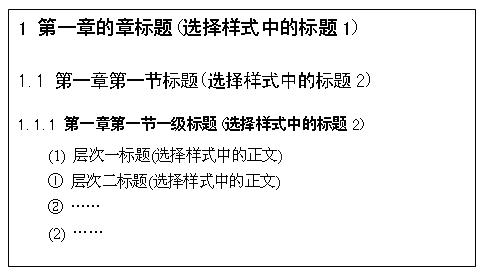
\includegraphics[scale=1]{figures/title.jpg}
	\caption[fig:chap1:title]{标题编号的示例}
\end{figure}

\section{各章之间的分隔符设置}{Section Headings}
各章之间应重新分页,使用“分页符”进行分隔。

设置方法:在“插入”菜单中选择“分隔符(B)…”,在弹出的窗口中选择分隔符类型为“分页符”,确定即可另起一页。

\section{正文中的编号}{Section Headings}

正文中的图、表、附注、公式一律采用阿拉伯数字分章编号。

如图1.2,表2.3,附注4.5,式6.7等。如“图1.2”就是指本论文第1章的第2个图。文中参考文献采用阿拉伯数字根据全文统一编号,如文献[3],文献[3,4],文献[6-10]等,在正文中引用时用右上角标标出。附录中的图、表、附注、参考文献、公式另行编号,如图A1,表B2,附注B3,或文献[A3]。


%%   - Chapter II
\input{body/chapter2}


%% if endnotes then
\printpagenotes


%% if a bibliography then
\renewcommand\bibname{参~考~文~献}
\bibliographystyle{gbt-7714-2015-numerical}
\bibliography{}

%% if appendices, then
\appendix
% \chapterstyle{dlutappendix}
\chapter{附录1}{Example 1}
...

\backmatter
%% if Biographical sketch then
% \begin{biosketch} ... \end{biosketch}

\end{document}
